Negli ultimi anni, la grande presenza di dipositivi in grado di catturare la posizione di un oggetto nel
tempo e le sue variazioni hanno prodotto enormi quantità di dati.
L'analisi di questi dati, resa possibile dalle moderne tecnologie Big Data, apre molteplici possibilità, come
ad esempio la ricerca dei flussi di traffico all'interno di un terriorio cittadino, oppure l'individuazione
dei luoghi più visitati da una certa categoria di utenti, o ancora il riconoscimento di gruppi di oggetti che si
muovono assieme all'interno di un certo spazio e tempo.
Dato il grande numero di potenziali fonti per i dati, è necessario ricondurre questi ultimi a una formulazione comune
così da poter sfruttare al meglio le loro potenzialità espressive.
La rappresentazione più basilare consiste nel considerare una traiettoria come l'insieme delle posizioni
spaziali dei punti che la compongono associando a ciascuno l'istante temporale in cui è stato registrato.
Questa formulazione prende il nome di traiettoria grezza (\textit{raw trajectory}), vedi~\cref{fig:chap-1:trajectory}
Andando a formalizzare quanto detto sopra:

\begin{figure}
  \centering
  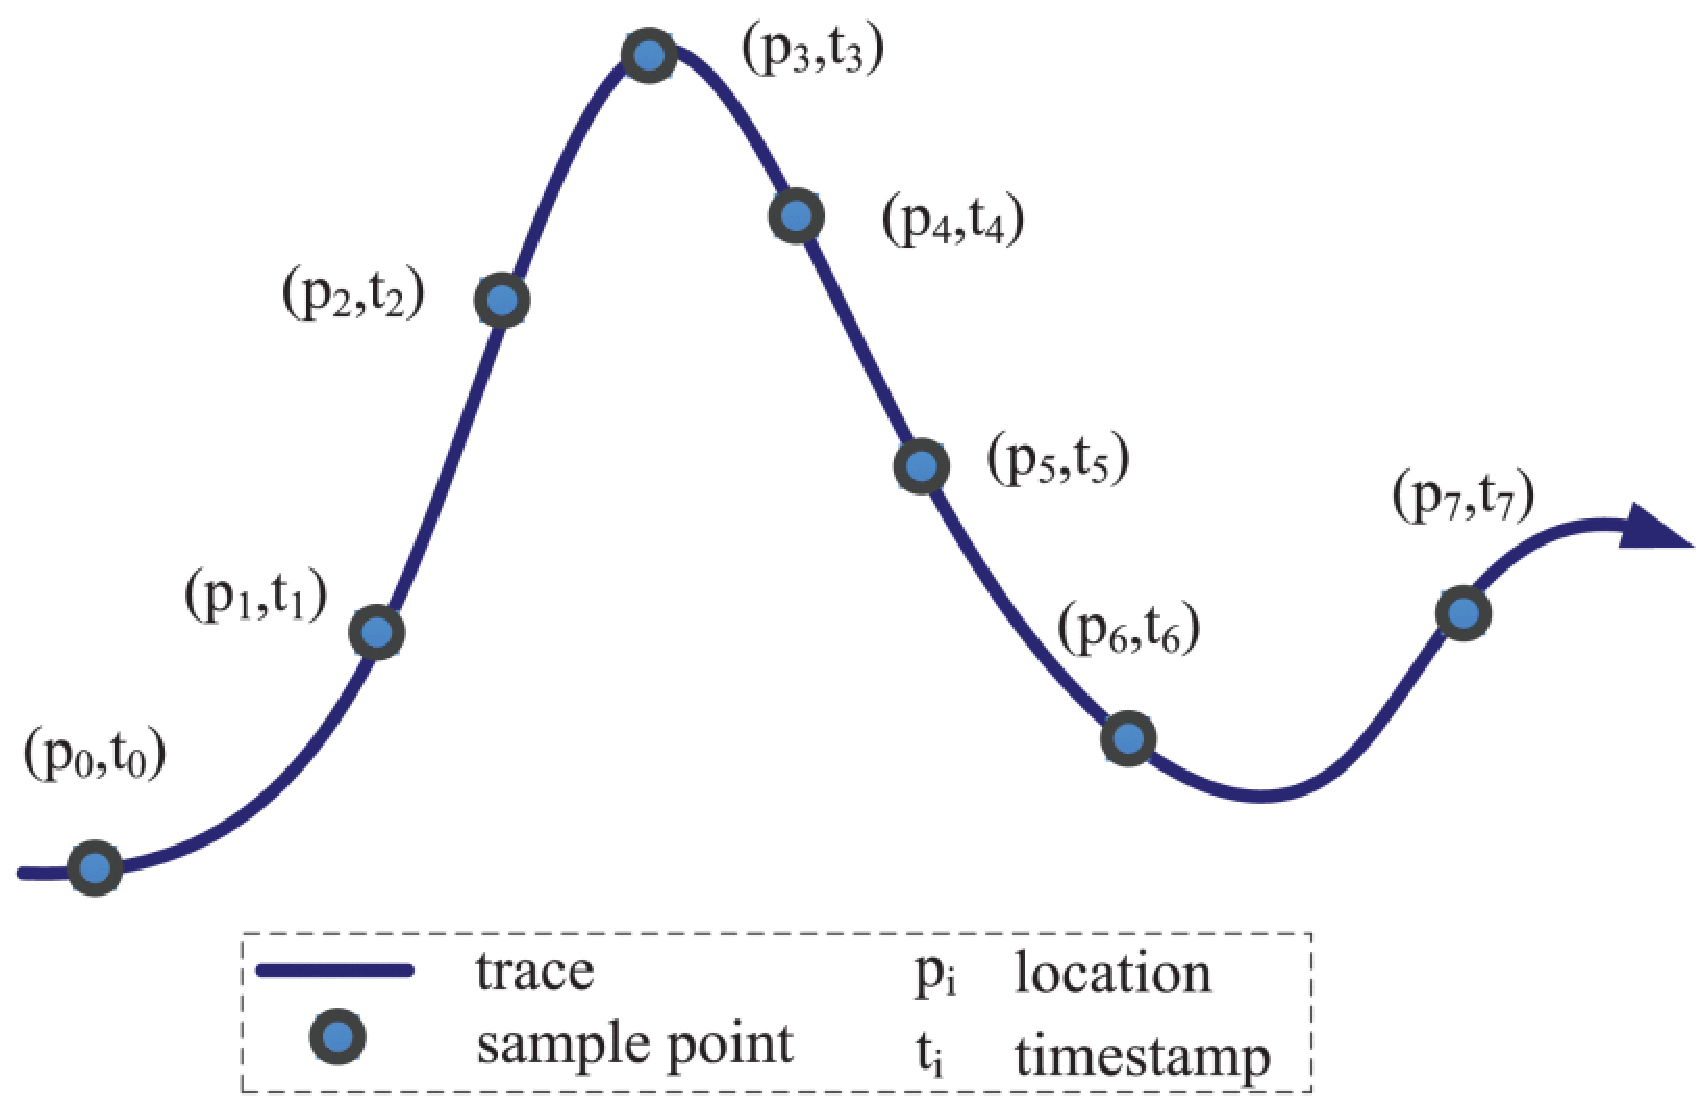
\includegraphics[scale=.5]{/sec-1/trajectory.pdf}
  \caption{Esempio di traiettoria,Fonte:\url{https://www.semanticscholar.org/paper/A-Survey-on-Trajectory-Data-Mining\%3A-Techniques-and-Feng-Zhu/a32f521442a540a6d1420526eaa68b3cab6b1d0d}}%
  \label{fig:chap-1:trajectory}
\end{figure}

\begin{definition}[Traiettoria]

  Si definisce una traiettoria grezza, o \textit{raw trajectory}, una sequenza temporale di punti \({p_{t}, p_{t'},\ldots, p_{t''}}\)
  tale che ogni punto \(p_{t}\) è composto da una coppia di coordinate spaziali \((latitude, longitude)\) e un tempo~\(t\).

\end{definition}

Questa basilare e semplice modalità di espressione può essere successivamente complicata, ad esempio adottando
una scala unica tra le diverse traiettorie per lo spazio e una per il tempo, oppure aggiungendo ulteriori informazioni, come ad esempio la direzione o attributi
dell'oggetto che la genera.

Per aumentare l'espressività della singola traiettoria, può essere utile definire il concetto di sotto-traiettoria, o \textit{subtrajectory}.
Intuitivamente una sotto-traiettoria non è altro che un segmento di una traiettoria relativo a un certo sottoinsieme dello spaziotempo coperto da quest'ultima.

\begin{definition}[Sottotraiettoria]

  Date due traiettorie \(TR\textsubscript{i}, TR\textsubscript{j}\) si definisce  \(TR\textsubscript{i}\) sottotraiettoria di \(TR\textsubscript{j}\) se \(\forall p_{t\textsubscript{i}} \in TR\textsubscript{i}, p_{t\textsubscript{i}} \in TR\textsubscript{j}\).

\end{definition}

Una volta definito che cos'è un dato di traiettoria, occorre mettere in chiaro che cosa distingue una traiettoria da un'altra.
Prendendo ad esempio il problema del clustering, sarebbe sbagliato tentare di applicare le stesse metriche di similarità anche ai dati di traiettoria
poiché gli oggetti in movimento producono spesso dati ad alta dimensionalità e con particolari correlazioni tra le dimensioni.
Il problema risulta quindi decisamente articolato: uno buona metrica di similarità deve tenere conto non solo dei singoli punti, ma anche della
traiettoria nella sua interezza, considerando anche la diversa lunghezza tra i due soggetti del confronto.
In letteratura sono presenti diversi metriche che possono essere impiegate nel confronto tra traiettorie:

\begin{itemize}

  \item \textbf{Distanza Euclidea.}
  La più semplice tra tutte le misure di stanza presentate, grazie alla sua complessità lineare permette di gestire dati ad alta dimensionalità.
  Date due traiettorie  \(T\textsubscript{i}\) e  \(T\textsubscript{j}\) di lunghezza \(n\) e dimensioni \(p\), la loro distanza euclidea si definisce come:

  \begin{equation}
    {D_E(T_{i}, T_{j}) = { {\frac{1}{n} } \sum_{k=1}^{n} {\sqrt{\sum_{m=1}^{p}{(a_{k}^{m} - b_{k}^{m})}^2}}}}
  \end{equation}

  La metrica tuttavia non è esente da difetti: è molto sensibile al rumore e richiede che le traiettorie siano uguali per numero di punti
  e dimensioni, inoltre anche l'intervallo di campionamento temporale deve coincidere. Questi limiti sono abbastanza difficili da
  aggirare quando si processa un dataset reale.

  Per superare questi problemi, sono disponibili diverse varianti della distanza euclidea: una su tutte è la \textit{Principal Component Analysis Plus Euclidean Distance} (PCA + distance)~\cite{zhang2006comparison}.
  Questa tecnica prima riduce le dimensioni spaziali ad una sola, successivamente esegue un'analisi PCA per convertire ogni traiettoria in
  \textit{k} coefficenti; a questo punto viene calcolata la distanza euclidea considerando i valori dei coefficenti individuati dall'analisi.
  Questa variazione mantiene gli stessi punti di forza della versione base della metrica, in più consente una maggior resistenza al rumore.



  \item \textbf{Distanza di Hausdorff.}
  La distanza di Hausdorff~\cite{chen2011clustering} misura quanto due traiettorie sono distanti l'una dall'altra.
  Date due traiettorie, per ogni punto di una viene calcolato il più vicino punto dell'altra e la distanza tra i due, il valore della distanza di Hausdorff
  corrisponde alla massima distanza calcolata nel passo precedente.~\cref{def:Hausdorff}
  \begin{equation} \label{def:Hausdorff}
    {D_{Hausdorff}(T_{i}, T_{j}) = \max{(h(T_{i}, T_{j}), h(T_{j}, T_{i}))}}~where~{h(T_{i}, T_{j}) = \max_{a \in T_{i}}{(\min_{b \in T_{j}}{(dist(a,b))})}}
  \end{equation}

  Nella formula \(h\) rappresenta la distanza di Hausdorff diretta, mentre \(d\) la distanza euclidea tra due punti.
  Il calcolo di entrambe le distanze dirette permette di gestire traiettorie con numero di punti differente tra loro.
  Questa metrica risulta robusta rispetto all'influenza causata da particolari distribuzioni di punti, ma allo stesso tempo è sensibile
  al rumore. Dalla formula~\cref{def:Hausdorff} è possibile definire la complessità computazionale della metrivca come \(O(m*n)\).


  \item \textbf{Distanza LCSS.}
  Longest Common Sub Sequence~\cite{rick2000efficient} affronta il problema con un approccio diverso: invece che calcolare la distanza fra i punti tra le due traiettorie, computa la
  più lunga sotto-sequenza.
  La lunghezza di quest'ultima determina la vicinanza,: più il valore è alto più le due traiettorie sono vicine.
  Essendo impossibile una coincidenza assoluta dei punti tra due traiettorie sono definite due soglie, \(\epsilon \) e \( \sigma \) che rispettivamente
  modellano la tolleranza rispetton all'asse x e y.
  LCSS può essere calcolata in modo ricorsivo, il suo tempo di computazione coincide con la diatnza di Hausdorff, inoltre consente una certa tolleranza rispetto
  alle deviazioni nei dati, ciò consente una buona efficenza nei dataset reali. Il maggior limite della metrica sta nella definizione dei parametri
  \(\epsilon \) e \( \sigma \) in problemi complessi.

  \item \textbf{Distnza DTW.}
  Dynamic time warping (DWT)~\cite{chen2005robust} pone il focus sulla dimensione temporale rispetto a quelle spaziali, come accadeva nelle metriche precedenti.
  Lo scopo è trovare l'allineamento ottimo tra due traiettorie dati certi vincoli.
  DWT resiste bene alle differenti lunghezze tra traiettorie: obbiettivo della misura è infatti ricercare il percorso a cui assimilare le traiettorie che abbia il minor coeficcente di distorsione,
  calcolato sulle trasformazioni subite dalle traiettorie.
  DWT assicura il rispetto dell'ordine tra i punti delle traiettorie, inoltre introducendo un principio di scaling locale della dimensione temporale,
  riesce a gestire scale temporali differenti tra le traiettorie.
  Tuttavia richiede continuità all'interno dei punti, è sensibile al rumore e a sottotraiettorie molto distanti tra loro.
  La complessità di questa misura è \(O(m*n)\).


  \item \textbf{Distanza di Fréchet.}
  La metrica di Fréchet~\cite{khoshaein2013trajectory} considera in contemporanea sia la dimensione temporale
  che quella spaziale durante il calcolo della distanza.
  Date due traiettorie di uguale lunghezza \(n\), si calcola la distanza euclidea tra i punti aventi stessa posizione all'interno delle due traiettorie:
  il valore più alto corrisponde alla distanza di Fréchet.
  Qualora le due traiettorie divergano come dimensioni, si eseguirà questo calcolo su tutte le possibili sotto-traiettorie di lunghezza \(n\) generabili
  dalla traiettoria più lunga.
  La complessità della misura nel caso peggiore è \(O(m*n)\).
  La distanza di Fréchet considera la traiettoria nella sua continuità, per questo motivo è molto sensibile agli outlier.


\end{itemize}



